%%%%%%%%%%%%%%%%%%%%%%%%%%%%%%%%%%%%%%%%%%%%%%%%%%%%%%%%%%%%%%%%%%%%
%%%%% HEADER %%%%%
%%%%%%%%%%%%%%%%%%%%%%%%%%%%%%%%%%%%%%%%%%%%%%%%%%%%%%%%%%%%%%%%%%%%

\documentclass[a4paper]{article}


%%%%% Packages %%%%%

	%%%%% Language %%%%% 
\usepackage[frenchb]{babel}
\usepackage[utf8]{inputenc}
\usepackage[T1]{fontenc}
	%%%%% Graphic %%%%%
\usepackage{graphicx}
	%%%%% Mise en page %%%%%
\usepackage{fancyhdr}

%%%%% Macros %%%%
\newcommand{\HRule}{\rule{\linewidth}{0.5mm}}

\pagestyle{fancy}
\lhead{\textsc{MiniEd} \\ Projet de Génie Logiciel}
\rhead{Coraline \textsc{Marie} \\ Vincent \textsc{Raveneau}}

%%%%% Doc's informations %%%%%


%%%%%%%%%%%%%%%%%%%%%%%%%%%%%%%%%%%%%%%%%%%%%%%%%%%%%%%%%%%%%%%%%%%%
%%%%% DOCUMENT %%%%%
%%%%%%%%%%%%%%%%%%%%%%%%%%%%%%%%%%%%%%%%%%%%%%%%%%%%%%%%%%%%%%%%%%%%

\begin{document}

	%%%%% Page de garde %%%%%%%%%%%%%%%%%%%%%%%%%%%%%%%%%%%%%%%%%%%%
	%%%%%%%%%%%%%%%%%%%%%%%%%%%%%%%%%%%%%%%%%%%%%%%%%%%%%%%%%%%%%%%%

	\begin{titlepage}
		\begin{center}

			% Logo et Université
			
\includegraphics[width=0.45\textwidth]{UN-sciences.png}~\\[2cm]

			\LARGE{Master 1 \sc{Alma}}\\[1.5cm]

			\Large{Projet de Génie Logiciel}\\[0.5cm]

			% Titre
			\HRule \\[0.4cm]
			{ \huge \bfseries \textsc{MiniEd} : Version 3 \\[0.4cm] }
			\HRule \\[1.5cm]

			% Auteur et Encadrant
			\normalsize		
			\emph{\'Etudiants :}\\
			Coraline \textsc{Marie} et Vincent \textsc{Raveneau}\\
			\vspace{0.5cm}
			\emph{Intervenant :} \\
			Gerson \textsc{Sunyé}
		
			\vfill

			% Date
			{\large 13 décembre 2013}

		\end{center}
	\end{titlepage}


	%%%%% Sommaire %%%%%%%%%%%%%%%%%%%%%%%%%%%%%%%%%%%%%%%%%%%%%%%%%
	%%%%%%%%%%%%%%%%%%%%%%%%%%%%%%%%%%%%%%%%%%%%%%%%%%%%%%%%%%%%%%%%

	\renewcommand{\contentsname}{Sommaire}
	\tableofcontents
	\newpage


	%%%%% Introduction %%%%%%%%%%%%%%%%%%%%%%%%%%%%%%%%%%%%%%%%%%%%%
	%%%%%%%%%%%%%%%%%%%%%%%%%%%%%%%%%%%%%%%%%%%%%%%%%%%%%%%%%%%%%%%%

	\begin{center}
		\section{Introduction}
	\end{center}

	\vspace{0.5cm}

	Le Génie Logiciel est la discipline qui permet l’aboutissement d’un projet depuis son idée, jusqu’à son utilisation par un client. Cette discipline est donc indispensable car elle est à l’origine de tout logiciel, et permet sa conception de façon fiable et structurelle.

	\vspace{0.5cm}

	Actuellement en première année de Master \textsc{Alma} à l’Université de Nantes, nous avions pour projet de Génie Logiciel, la conception d’un éditeur de texte simplifié. Cet éditeur basique : \textsc{MiniEd}, devait disposer de diverses fonctionnalités, qui ont été développées dans trois versions différentes du logiciel.  

	\vspace{0.5cm}

	Ce rapport présente donc la conception de \textsc{MiniEd}, au travers de ses trois versions fonctionnelles. Ces différentes versions disposent chacune de fonctionnalités et de commandes basiques, qui ont eu comme objectifs pédagogiques de nous sensibiliser sur le rôle du Génie Logiciel dans l'Informatique.

	\vspace{2.5cm}

	\begin{center}
		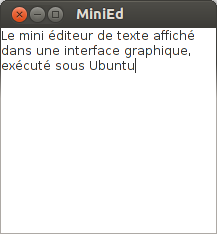
\includegraphics[width=0.5\textwidth]{MiniEd_capture.png}~
	\end{center}

	\newpage


	%%%%% Partie 1 %%%%%%%%%%%%%%%%%%%%%%%%%%%%%%%%%%%%%%%%%%%%%%%%%
	%%%%%%%%%%%%%%%%%%%%%%%%%%%%%%%%%%%%%%%%%%%%%%%%%%%%%%%%%%%%%%%%

	\begin{center}
		\section{Conception}
	\end{center}

	\vspace{0.5cm}

		%%%%% Partie 1.1 %%%%%%%%%%%%%%%%%%%%%%%%%%%%%%%%%%%%%%%%%%%
		\subsection{Dépendances externes}

		\vspace{0.5cm}

		Avant même de concevoir un logiciel, il faut au préalable le penser, ainsi que définir ses besoins et ses différentes fonctionnalités. Dans cette optique, notre cahier des charges nous imposait de concevoir l’éditeur de texte dans le langage de programmation Scala, un langage récent qui allie de façon subtile la programmation orientée objet avec la programmation fonctionnelle. Ce langage ne fût pas choisi pour ses performances en programmation orientée objet, mais plutôt dans une optique pédagogique, car nous ne l'avions encore jamais utilisé avant le projet \textsc{MiniEd}.

		\vspace{0.5cm}

		Dans un soucis de fiabilité, de qualité et de performances, le code de l'éditeur de texte a été testé à l'aide de JUnit. Ce dernier est un framework de test unitaire qui fût créé pour le langage de programmation Java, et qui est aujourd’hui compatible avec le langage de programmation Scala.

		\vspace{0.5cm}

		Le cahier des charges de \textsc{MiniEd} nous demandait de modéliser une interface homme-machine. Dans un soucis d'esthétique, cette dernière est de type graphique, ce qui la rend plus intuitive et plus agréable pour les utilisateurs. Ainsi, pour concevoir l'interface, nous avons fait appel à la bibliothèque Java Swing qui est une bibliothèque graphique pour Java.

		\vspace{0.5cm}

		%%%%% Partie 1.2 %%%%%%%%%%%%%%%%%%%%%%%%%%%%%%%%%%%%%%%%%%%
		\subsection{Fonctionnalités du logiciel}

		\vspace{0.5cm}

		Le cahier des charges de \textsc{MiniEd} réclamait plusieurs fonctionnalités, qui ont été développées sur plusieurs versions fonctionnelles de l'éditeur. La programmation s'est donc déroulée en trois étapes : trois versions de \textsc{MiniEd}.

		\vspace{0.5cm}

			%%%%% Partie 1.2.1 %%%%%
			\subsubsection{Version 1 : Les actions de base}

			Les actions de base de \textsc{MiniEd}, sont celles qui ont été mises en place pour la première version du logiciel. Comme on peut s'y attendre, celles-ci sont fondamentales et sont :

			\begin{itemize}
				\item La saisie de texte.

				\item Les actions Couper, Copier, Coller et Effacer.

				\item L'implémentation d’un buffer qui est notre zone de travail, et dans lequel est contenu le texte.

				\item La mise en place de la sélection qui donne la possibilité de sélectionner une partie, voire même la totalité du texte. Ainsi, le texte sélectionné peut être retravaillé à l’aide d’autres fonctionnalités.

				\item L’implémentation d’un presse-papier qui contient du texte que l’on a au préalable, couper ou copier, et qui peut ensuite être collé.

				\item La création de macros qui groupe certaines commandes utilisateur. Dans notre cas cette fonctionnalité était l'un des objectifs de la version 1, mais nous n'avons pas eu le temps de la mettre en place avant la version 2.

				\item La conception d’une interface homme-machine qui est de type graphique. Plusieurs interfaces peuvent être générées et elles sont toutes associées au même buffer.
			\end{itemize}

			%%%%% Partie 1.2.2 %%%%%
			\subsubsection{Version 2 : L'enregistrement des actions de l'utilisateur}

			Pour la seconde version de \textsc{MiniEd}, le cahier des charges nous demandait de développer une nouvelle fonctionnalité. Il s'agissait de permettre l'enregistrement de toutes les actions de l'utilisateur, de façon à pouvoir les rejouer à volonté.

			%%%%% Partie 1.2.3 %%%%%
			\subsubsection{Version 3 : Le défaire / refaire}

			Enfin, la dernière fonctionnalité qui a été mise en place est le défaire / refaire. Il s'agit de l'équivalent des commandes "annuler" et "rétablir" que l'on trouve sur d'autres éditeurs de texte. Grâce à cette fonctionnalité, l'utilisateur peut désormais annuler pas à pas, toutes les actions qu'il a fait depuis le lancement de \textsc{MiniEd} (défaire), et s'il le souhaîte, il peut ensuite rétablir ce qu'il vient de défaire (refaire).

			\vspace{0.5cm}

		%%%%% Partie 1.3 %%%%%%%%%%%%%%%%%%%%%%%%%%%%%%%%%%%%%%%%%%%
		\subsection{Schématisation}

		\vspace{0.5cm}

		Dans un soucis de clarté et de compréhensibilité de notre cahier des charges, voici un diagramme de classe décrivant la structure de notre application. Dans ce diagramme sont schématisées les classes nécessaires au bon fonctionnement de l’éditeur de texte ainsi que leurs dépendances. Nous y avons rajouté les pattern que nous avons utilisé.

	\begin{center}
		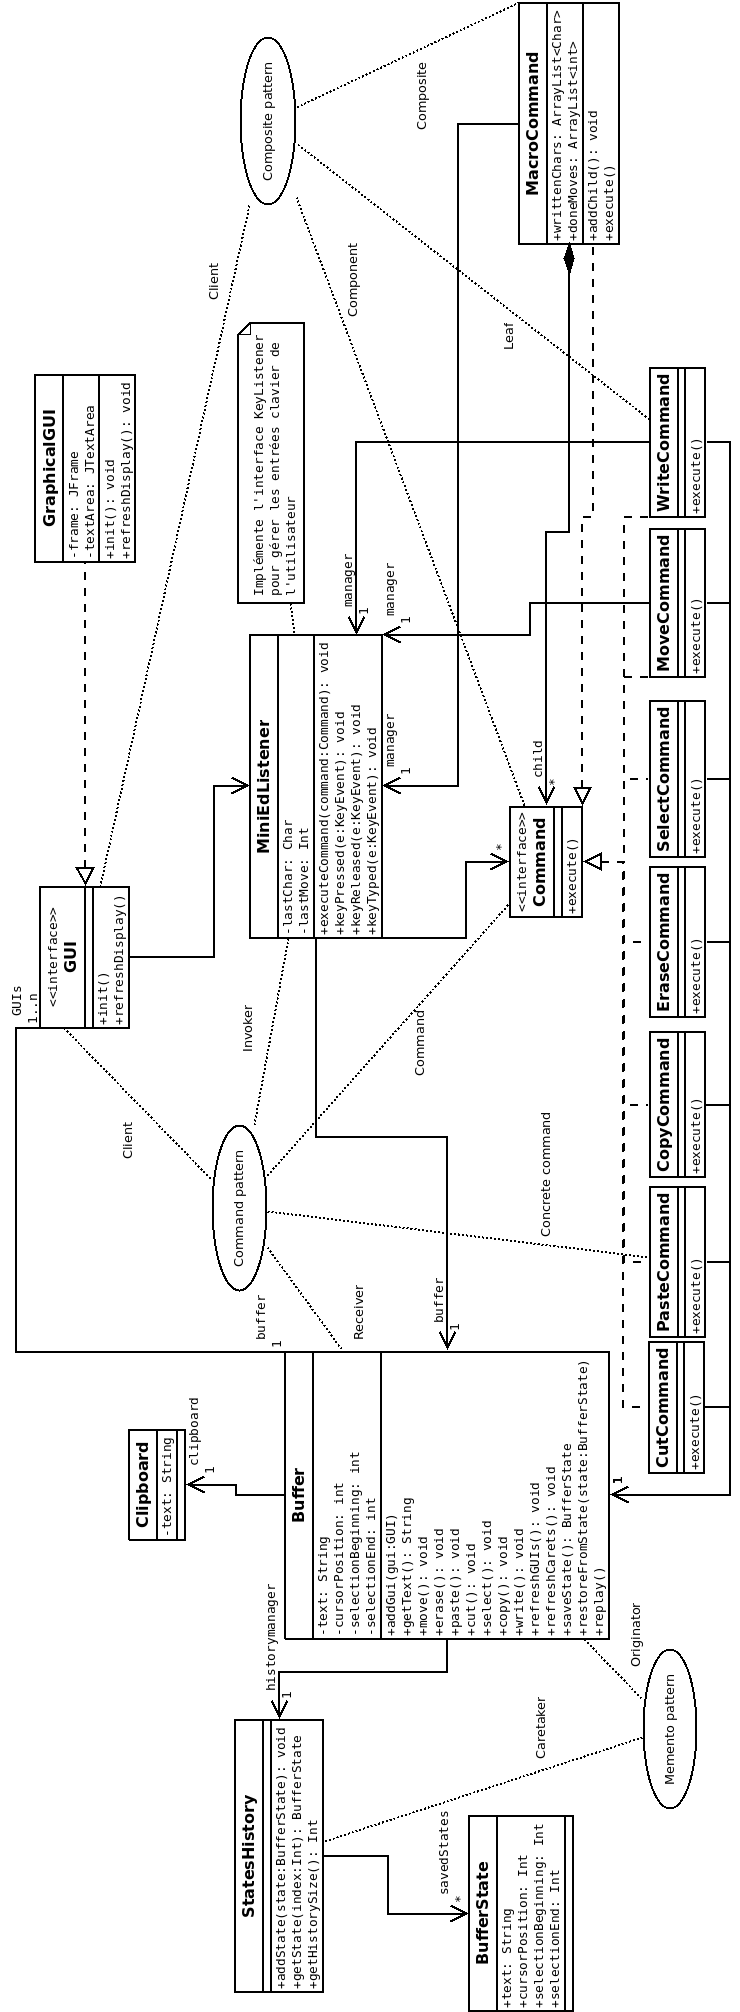
\includegraphics[width=0.9\textwidth]{UML.png}~
	\end{center}

		De plus, pour illustrer la commande la plus importante du logiciel, nous avons créé un diagramme de séquence sur la commande \texttt{Write}.

	\begin{center}
		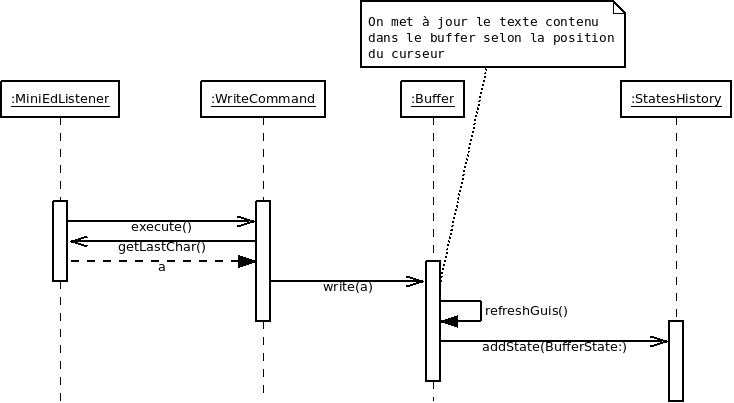
\includegraphics[width=0.9\textwidth]{WriteSeq.png}~
	\end{center}
	\newpage
	

	%%%%% Partie 2 %%%%%%%%%%%%%%%%%%%%%%%%%%%%%%%%%%%%%%%%%%%%%%%%%
	%%%%%%%%%%%%%%%%%%%%%%%%%%%%%%%%%%%%%%%%%%%%%%%%%%%%%%%%%%%%%%%%

	\begin{center}
		\section{Développement du logiciel}
	\end{center}

	\vspace{0.5cm}

		%%%%% Partie 2.1 %%%%%%%%%%%%%%%%%%%%%%%%%%%%%%%%%%%%%%%%%%%
		\subsection{Les classes}

		\vspace{0.5cm}

		Comme il est possible de le voir sur le diagramme UML précédent, l'éditeur de texte est relativement complexe, et composé de multiples classes. 

		\vspace{0.5cm}

			%%%%% Partie 2.1.1 %%%%%
			\subsubsection{L'interface graphique}

			L'interface graphique est composée par quatre classes :

			\begin{itemize}
				\item Les classes \texttt{GUI}, et \texttt{GraphicalGUI} qui composent l'interface graphique (gestion de la fenêtre \dots)

				\item Les classes \texttt{MiniEdListener} et \texttt{TextualGUI} qui s'occupent de l'interface textuelle (traitement des entrées clavier \dots)
			\end{itemize}

			%%%%% Partie 2.1.2 %%%%%
			\subsubsection{Les commandes}

			En ce qui concerne les commandes de l'éditeur de texte, elles ont chacune leur propre classe dépendante de la classe abstraite \texttt{Command}.

			\begin{itemize}
				\item La classe \texttt{CutCommand} : appelle la méthode \texttt{cut} de la classe \texttt{Buffer}

				\item La classe \texttt{PasteCommand} : appelle la méthode \texttt{paste} de la classe \texttt{Buffer}

				\item La classe \texttt{MoveCommand} : appelle la méthode \texttt{move} de la classe \texttt{Buffer}

				\item La classe \texttt{EraseCommand} : appelle la méthode \texttt{erase} de la classe \texttt{Buffer}

				\item La classe \texttt{SelectCommand} : appelle la méthode \texttt{select} de la classe \texttt{Buffer}

				\item La classe \texttt{CopyCommand} : appelle la méthode \texttt{copy} de la classe \texttt{Buffer}

				\item La classe \texttt{WriteCommand} : appelle la méthode \texttt{write} de la classe \texttt{Buffer}
			\end{itemize}

			%%%%% Partie 2.1.3 %%%%%
			\subsubsection{Le buffer}

			La classe \texttt{Buffer} permet de gérer le texte de l'éditeur.

			%%%%% Partie 2.1.4 %%%%%
			\subsubsection{Le presse-papier}

			La classe \texttt{Clipboard} offre les fonctionnalités d'un presse-papier et permet ainsi le coupage, la copie et le collage d'une sélection de texte.

			%%%%% Partie 2.1.5 %%%%%
			\subsubsection{Macros et enregistrement}

			Les macros et l'enregistrement des actions de l'utilisateur sont gérées par les classes \texttt{MacroCommand}, \texttt{BufferState} et \texttt{StatesHistory}. Celles-ci permettent de mettre en place la gestion des macros utilisateur, et d’enregistrer les actions effectuées par celui-ci. Les macros sont une suite de commandes que l’utilisateur pourra définir lors de l’utilisation du logiciel, afin de les rejouer plus tard. Ici, elles sont appelées via le raccourci \texttt{ctrl + M}, qui fonctionne de la façon suivante :

			\begin{itemize}
				\item Le premier appel permet de débuter l’enregistrement de la macro.

				\item Le deuxième appel permet de terminer l’enregistrement de la macro. Toute action effectuée par l’utilisateur depuis le début de l’enregistrement est ainsi contenue dans la macro.

				\item Les appels suivants exécutent le contenu de la macro à l’emplacement du pointeur.
			\end{itemize}

			L’enregistrement des actions de l’utilisateur est également effectué automatiquement tout au long de l’exécution du programme. Ces actions peuvent être rejouées avec le raccourci \texttt{ctrl + P}. Cependant, aucun changement visuel ne se produit lors de cette action, le temps nécessaire à l’ordinateur pour rejouer les actions étant bien trop faible pour que l’action soit perçue.

			%%%%% Partie 2.1.6 %%%%%
			\subsubsection{Défaire / Refaire}

			Les fonctionnalités de défaire / refaire sont accessible grâce à deux classes : \texttt{UndoCommand} et \texttt{RedoCommand}. Elles permettent à l'utilisateur de revenir en arrière, c'est à dire d'annuler chaque étape de saisie jusqu'au début, ou de rétablir ce que l'utilisateur vient de défaire.

		\vspace{0.5cm}

		%%%%% Partie 2.2 %%%%%%%%%%%%%%%%%%%%%%%%%%%%%%%%%%%%%%%%%%%
		\subsection{Patrons de conception}

		\vspace{0.5cm}

		Afin de concevoir notre logiciel, nous avons utilisé plusieurs Design Pattern :

		\vspace{0.5cm}

		Le premier Pattern que nous utilisons est le Pattern Commande. Celui-ci est un patron de conception de type comportemental qui encapsule la notion d'Invocation. Il permet de séparer le code de l'appel des commandes, avec le code des commandes elles-mêmes.

		\vspace{0.5cm}

		Le second Pattern que nous utilisons est le Pattern Composite. Ce pattern est un patron de conception structurel qui permet de simplifier l'utilisation de plusieurs objets similaires. Dans notre cas, nous avons utilisé le Pattern Composite pour concevoir une macro permettant la stockage de commandes.

		\vspace{0.5cm}

		Le troisième Pattern que nous utilisons est le pattern Memento. Il permet de conserver l’état d’un objet pour le restaurer ultérieurement. Ce Pattern a été utilisé afin de réaliser l’enregistrement des actions effectuées par l’utilisateur. En effet, à chaque action l’état du buffer est enregistré en mémoire, afin d'établir un historique.

		\vspace{0.5cm}

		%%%%% Partie 2.3 %%%%%%%%%%%%%%%%%%%%%%%%%%%%%%%%%%%%%%%%%%%
		\subsection{Tests et fiabilité}

		\vspace{0.5cm}

		Aujourd’hui, la qualité d’un logiciel se juge autant sur sa fiabilité que sur ses compétences. C’est pourquoi nous avons développé plusieurs classes de test améliorant la fiabilité de notre logiciel. Dans ce but, nous avons mis en place des tests unitaires à l’aide de JUnit, ce qui permet de tester le bon fonctionnement de nos classes et de leurs méthodes.

		\vspace{0.5cm}


	%%%%% Conclusion %%%%%%%%%%%%%%%%%%%%%%%%%%%%%%%%%%%%%%%%%%%%%%%
	%%%%%%%%%%%%%%%%%%%%%%%%%%%%%%%%%%%%%%%%%%%%%%%%%%%%%%%%%%%%%%%%

	\begin{center}
		\section{Conclusion}
	\end{center}

	\vspace{0.5cm}

	Malgré sa simplicité, \textsc{MiniEd} reste un projet d'apprentissage. Ce travail nous a donc enseigné plusieurs choses, comme par exemple le langage Scala, tout en nous permettant de mettre en application les différentes notions étudiées en Génie Logiciel. Nous avons conçu \textsc{MiniEd} depuis la base et mis en place les concepts d'UML, de multiclasses et de Design Pattern au service de notre programme.

	\vspace{0.5cm}

	De plus, le fait de séparer la conception en trois versions fonctionnelles de l'éditeur, nous a aidé à réaliser un logiciel fiable et performant. En effet, chaque version se devait d'être fonctionnelle et de répondre précisément au cahier des charges, ce qui impliquait une vérification et des tests pour chaque rendu. 

	\vspace{0.5cm}

	\textsc{MiniEd} nous a permis d’utiliser de nouvelles connaissances étudiées en Génie Logiciel, mais pas seulement. Nous nous sommes servis pour ce projet d'autres notions vues dans d’autres modules d'enseignement, comme \textit{Concepts et Outils de Développement}, ou \textit{Vérifications et Tests}.

\end{document}
